\subsection{Pure Native vs Hybrid Native vs Hybrid vs Web Apps}

The mobile app market is segmented into several platforms. Each platform has it’s own framework, API, and language specifications and requirements. Android apps are written in java and access the Android apis, iOS apps in Objective-C or Swift and interface with the iOS frameworks. Android and iOS cover about 94\% of the worldwide mobile market \cite{mobile_market}. A developer must de decide which platforms are priorities, and how might programming effort be consolidated across multiple platforms. Several strategies exist, and there are many tool kits and frameworks that can help accelerate development.

\begin{itemize}[label={}]

\item \textbf{Web Apps}: The simplest development strategy is to develop an HTML based web page that is disguised to appear and behave like a mobile app. The web app runs in a normal browser, is deployed from a standard web server. Model mobile web browsers offer javascript APIs that can access various other hardware components of the smart phone such as the compass, GPS/geolocation services, accelerometer, and the camera. Other services will remain inaccessible.

\item \textbf{Hybrid}: A similar strategy is to develop using javascript and html, but to package these elements into a “hollow” native app that is little else than a native view component with an embedded web browser. The web browser url is locked to the internal html files and appears to the user as a mobile app. though the user interface might slightly different that a pure native app. The advantage of a hybrid strategy is that the app can be distributed via the standard app stores increasing it’s marketability. It can also be extended with native components that might otherwise not be accessible to to a web app such as internal file storage and native data storage mechanisms.

\item \textbf{Pure Native}: The developer uses the development environment as provided by the phone manufacturer and has full access to all of the native hardware APIs, development kits and tools. The performance and responsiveness of a pure native app is much better compared to web and hybrid solutions. The user interface is build with the standard UI tools allowing a better user experience because the user is presented with familiar UI elements.

\item \textbf{Hybrid Native}: Recently several cross platform application frameworks and emerged that allow the developer in a single language that can be compiled across several platforms. Qt and Juce are examples of application frameworks that allow cross platform development in C++, Xamarin uses C\#.

\end{itemize}

The criteria to compare these strategies are the following:

\begin{itemize}[label={}]

\item \textbf{Development Effort }: Judging the development effort is subjective. It depends greatly on the experience of the developers involved. An expert Objective-C developer with years of experience developing IOS applications will have no problem developing a native IOS app, but might be stumped when it comes to hybrid development. For this project we will assume Javascript and HTML development requires the least amount of effort and thus give high scores to Web Apps and Hybrid development.

\item \textbf{Code Portability}: How much of the code developed can be reused on each target platform without any extra effort.

\item \textbf{Camera Access}: Does a strategy allow access to all the device’s camera,? is the camera view customisable with guidelines and information that can help the user take a high quality picture?


\item \textbf{Look and Feel}: Does a strategy offer pure native UI elements that conform with user expectations for a particular device?

\item \textbf{Deployment}: What effort is required to deploy the application to a device?

\item \textbf{Performance}: What is the performance impact of a chosen strategy?

\end{itemize}

For comparison we rank each criteria per strategy either 2 = benefit, 1 = no benefit, 0 = negative benefit.

\begin{figure}[H]
    \centering
    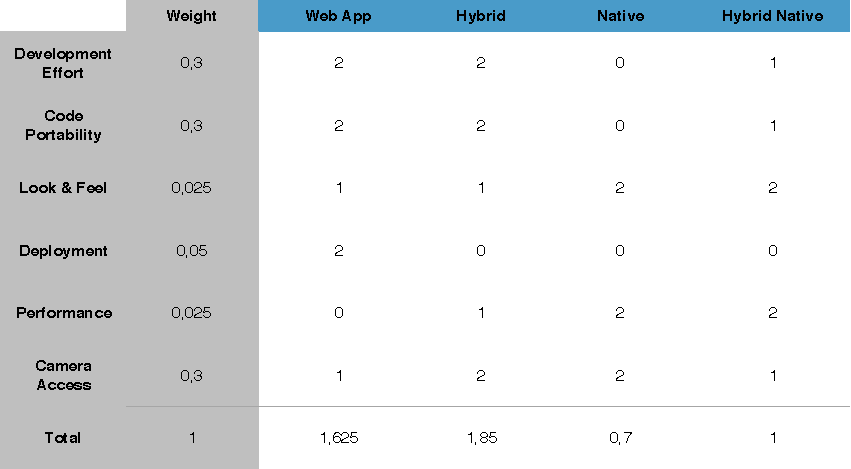
\includegraphics[height=8cm,keepaspectratio]{assets/concept/native_vs_hybrid.pdf}
    \caption{Mobile Development Strategies Comparison}
    \label{fig:mob_strat}
\end{figure}

